\section{The CAMS Framework}
The CARP Mobile Sensing (CAMS) Framework\footnote{\url{https://github.com/cph-cachet/carp.sensing-flutter/wiki}} is a Flutter framework for adding digital phenotyping capabilities to a mobile-health app. CAMS is designed to collect research-quality sensor data from the many smartphone data channels such as sensors and location data -in addition to external sensors which the phone is connected to, such as wearable devices.  

The core idea is to allow application programmers to design and implement a custom mobile health app without having to start from scratch, with regards to the sensor integration, by enabling the programmers to add mobile sensing capabilities in a 'flexible and simple' manner. This would include, firstly, adding support for collecting health-related data such as ECG, Location, Sleep, Activity, Step Count and much more. Secondly, to format this data according to different health data formats (like Open mHealth schemas \footnote{\url{https://www.openmhealth.org/documentation/#/schema-docs/schema-library}}); Thirdly, to use this data in the app and to upload it to a specific server, using a specific API (such as REST), in a specific format.

To include as many users as possible, the app should be cross-platform, i.e. available both on Android and iOS. To include as many data channels as possible the application should also be able to support different wearable devices for ECG monitoring and activity tracking. Hence, focus is on software engineering support in terms of a solid programming API and a runtime execution environment, that is being maintained as the underlying mobile phone operating systems and APIs are evolving. Moreover, the focus is on providing an extensible API and runtime environment, which together allow for adding application-specific data sampling, wearable devices, data formatting, data management, and data uploading functionality to an application.

\subsection{The CAMS Domain Model}
The data collection pipeline is the defined firstly by a \textbf{Study} which contains all the information needed to conduct a real-world study, which includes collection of certain data types with a set of rules and saving it somewhere. 

Concretely, a \textbf{Study} holds a set of \textbf{Triggers}, which define \textit{when} sampling is carried out, such as by scheduling sampling at  given time each day, or when a certain event is registered, such as entering a specific GeoFence. 

Each \textbf{Trigger} holds one or more \textbf{Tasks}, each of which define which \textbf{Measures} should run simultaneously. In addtion, a \textbf{Task} also defines whether or not data is sampled in the background, or whether the user needs to interact with the device in order to perform sampling. 

Each \textbf{Task} holds a set of \textbf{Measures} each of which define what to sample, i.e. which data channel to listen to. Lastly, a \textbf{Study} also holds a reference to the \textbf{DataEndpoint} specifying which where data ends up, i.e. by uploading it to a server.

\begin{figure}
    \centering
    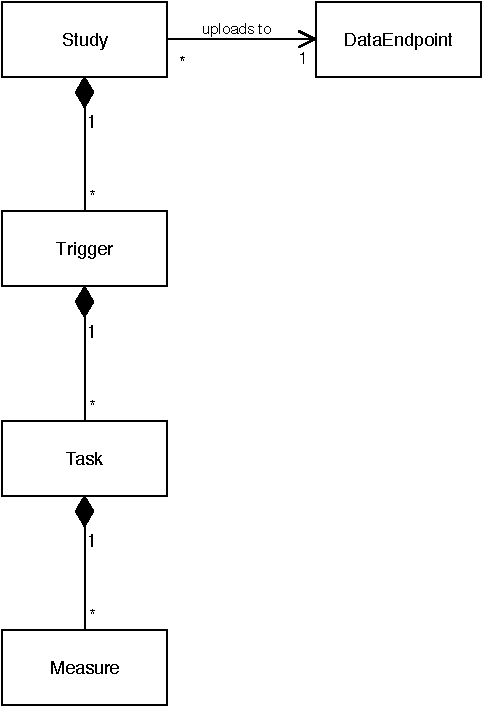
\includegraphics[width=0.5\textwidth]{images/CAMS.pdf}
    \caption{CAMS Domain Model}
    \label{fig:cams_uml}
\end{figure}

An integration for the CAMS Framework will be described later in this thesis. 